 \providecommand{\main}{../..}
\documentclass[\main/main.tex]{subfiles}
\begin{document}
\subsection{Esercizio 2.8}

\begin{figure}
  \begin{align*}
    \min z = x_2         \\
    1x_1 + 3x_2 & \leq 8 \\
    x_1 + 5x_2  & \leq 3 \\
    2x_1 - 2x_2 & \geq 7 \\
    3x_1 + 3x_2 & \geq 8 \\
    x_1, x_2    & \geq 0
  \end{align*}
  \caption{Esercizio 2.8}
\end{figure}

\subsection{Risoluzione esercizio 2.8}

\begin{figure}
  \begin{subfigure}{0.45\textwidth}
    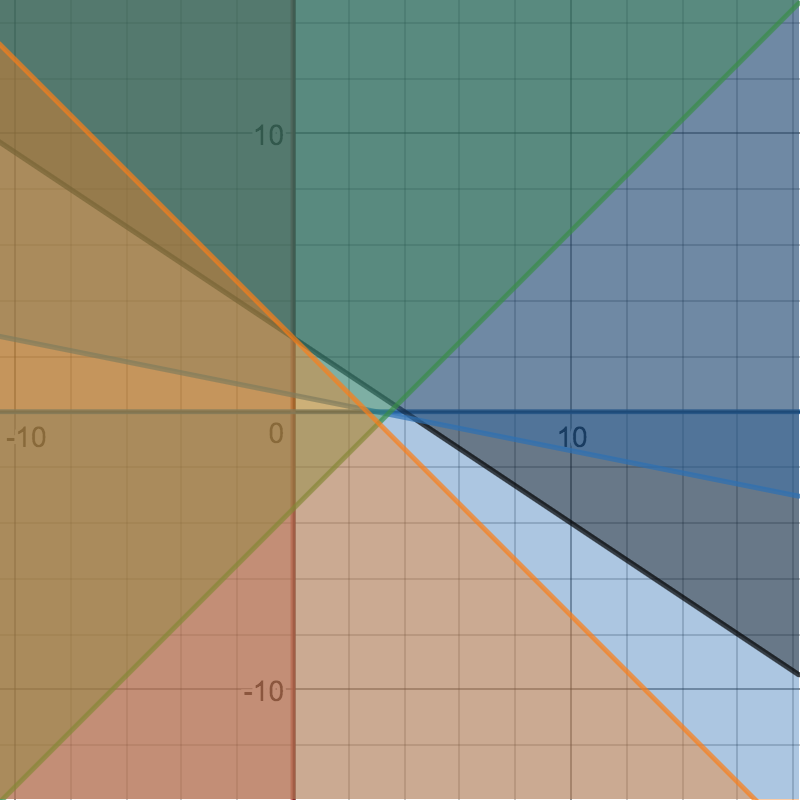
\includegraphics[width=0.8\textwidth]{2_8}
    \caption{I vincoli del problema nello spazio $x_1 - x_2$}
  \end{subfigure}
  \caption{Risoluzione esercizio 2.8}
\end{figure}

La regione ammissibile è vuota.

\end{document}